%--------------------------------------------------------------------
%
% file: cs446_pres.tex
%
% @Author  Iacovos G. Kolokasis
%          Emmanouil Pavlidakis
% @Version 13-05-2018
% @email   kolokasis@ics.forth.gr
%          manospavl@ics.forth.gr
% 
% @brief   Presentatin for the project needed of CS-445 Managed
% Runtime Systems project 

% The theme itself is licensed under a Creative Commons
% Attribution-ShareAlike 4.0 International License. This means that if
% you change the theme and re-distribute it, you must retain the
% copyright notice header and license it under the same CC-BY-SA
% license. This does not affect the presentation that you create with
% the theme.
%
% Downloaded from : https://github.com/matze/mtheme
%
%--------------------------------------------------------------------

%\documentclass[handout,....]{beamer}   % Disable beamer pause
\documentclass[10pt]{beamer}

\usetheme{metropolis}

%--------------------------------------------------------------------
% PACKAGES
%--------------------------------------------------------------------
\usepackage{appendixnumberbeamer}
\usepackage{tabularx}
\usepackage{booktabs}
\usepackage[scale=2]{ccicons}
\usepackage{pgfplots}
\usepgfplotslibrary{dateplot}
\usepackage{xspace}
\usepackage{listings}
\usepackage{adjustbox}      
\usepackage{textpos}
\usepackage{adjustbox} 
\usepackage{svg}

\usepackage{graphicx}

\newcommand{\themename}{\textbf{\textsc{metropolis}}\xspace}

\setbeamertemplate{footline}{
    \leavevmode%
    \begin{beamercolorbox}[left,wd=.4\paperwidth,ht=2.5ex,dp=1.125ex,leftskip=.3cm, rightskip=.3cm plus1fil]{footline}%
        \href{https://www.csd.uoc.gr/~hy446}{CS446 - Managed RunTime Systems}%
    \end{beamercolorbox}
    %
    \begin{beamercolorbox}[center,wd=.2\paperwidth,ht=2.5ex,dp=1.125ex,leftskip=.3cm,rightskip=.3cm plus1fil]{footline}%
        \centering
        \insertframenumber~\textlatin{of}~\inserttotalframenumber%
    \end{beamercolorbox}%
    %
    \begin{beamercolorbox}[right,wd=.4\paperwidth,ht=2.5ex,dp=1.125ex,leftskip=.3cm,rightskip=.3cm plus1fil]{footline}%
        \hskip2ex plus1fill%
        \href{mailto:manospavl@ics.forth.gr}{\textlatin{$[$ manospavl, }}%
        \href{mailto:kolokasis@csd.uoc.gr}{\textlatin{kolokasis $]$@ics.forth.gr}}
    \end{beamercolorbox}%
}%

%--------------------------------------------------------------------
% TITLE
%--------------------------------------------------------------------
\title{\textlatin{Evaluating the Performance of Interpreters\\Over Various Branch Predictors}}
\subtitle{CS-446 -- Managed Runtime Systems}
\date{\today}
\author{Emmanouil Pavlidakis \& Iacovos G. Kolokasis}
\institute{Computer Science Department \\ University Of Crete}
\titlegraphic{\hfill
\includegraphics[height=1.5cm]{figures/UoC_logo.png}}

%--------------------------------------------------------------------
% PRESENTATION SLIDES
%--------------------------------------------------------------------
\begin{document}

{
\maketitle
}

%--------------------------------------------------------------------
% TABLE OF CONTENTS
%--------------------------------------------------------------------
{
\begin{frame}{Contents}
  \setbeamertemplate{section in toc}[sections numbered]
  \tableofcontents[hideallsubsections]
\end{frame}
}

%--------------------------------------------------------------------
% INTRODUCTION
%--------------------------------------------------------------------
\section{Background \& Problem statement}

\begin{frame}{What are Interpreters?}
    \begin{itemize}
    	\item {Directly transforms \& executes program instructions written in a high-level programming language} 
    	\item {Two types of interpreters : }
    	\begin{enumerate}
    		\item {Transform the source code to machine code}
    		\item {Transform the source code to byte code}
    	\end{enumerate}	
        \item {Byte code can be generated: }
	         \begin{itemize}
	         	\item{Statically: Before actual execution (i.e. Java)}
	         	\item{Dynamically: Just before execution (i.e. Python)}
	         	\item{Dynamically: At runtime (i.e. Javascript))}
	         \end{itemize}
    \end{itemize}
    \begin{figure}
	    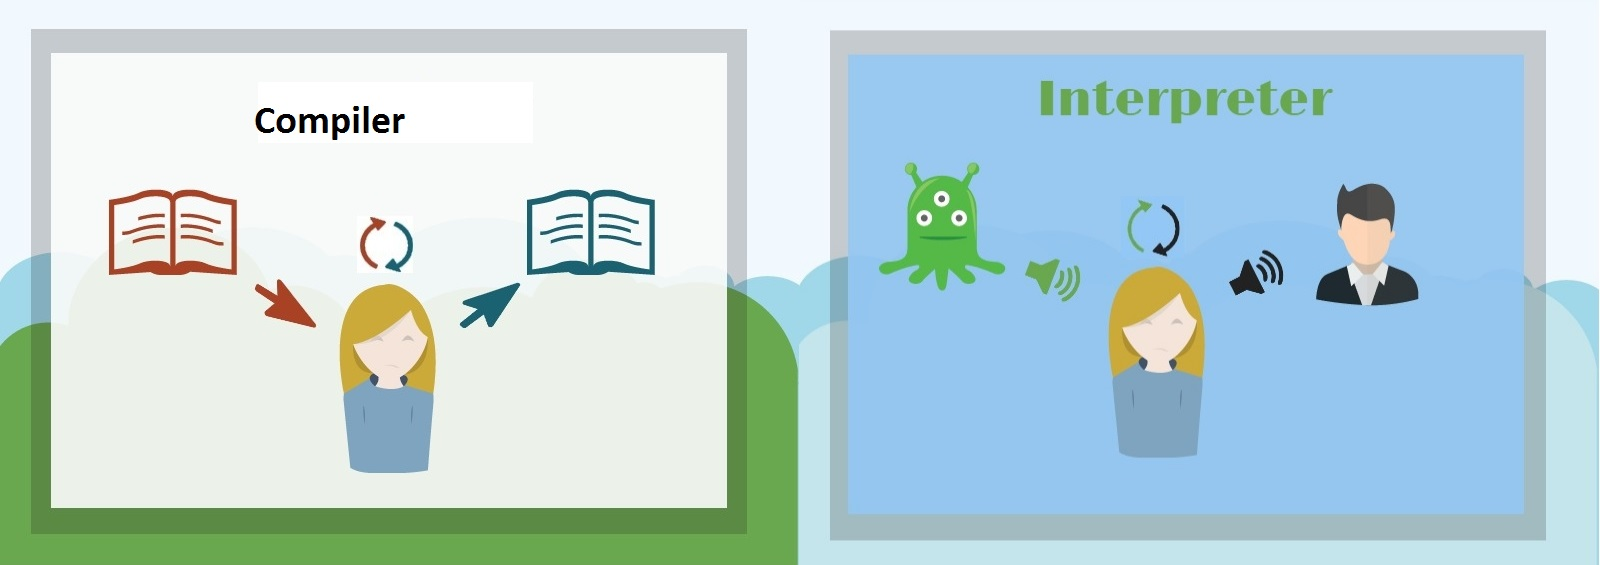
\includegraphics[height=1.5cm]{figures/interVSComp.jpg}
    \end{figure}
\end{frame}

\begin{frame}[fragile]{Performance Issues}
    \begin{columns}[T] % align columns
        \begin{column}{.65\textwidth}
            \begin{center}
                \begin{itemize}
                    \item {Interpreters contain an infinite loop}
                        \begin{itemize}
                            \item {Fetches, Decodes, and Executes commands}
                        \end{itemize}
                    \item {Their main overhead derives from this dispatch loop}
                    \item {Additional costs come from the switch st.}
                        \begin{itemize}
                            \item {They causes indirect jump instructions}
                            \item {These indirect branches are very difficult to predict}
                            \item {Every miss prediction costs almost 20 cycles}
                        \end{itemize}
                \end{itemize}
            \end{center}
        \end{column}%
            \hfill%
            \begin{column}{.35\textwidth}
                \metroset{block=fill}
                \begin{alertblock}{Dispatch Loop}
                    \begin{center}
                        \begin{lstlisting}[basicstyle=\footnotesize , breaklines]
while(1){
    opc = * vpc++;
    switch (opc) {
        case ADD:
        ....
        break;
        case  SUB:
        ....				
        break;
    }	
}
                        \end{lstlisting}
                    \end{center}
                \end{alertblock}
            \end{column}%
    \end{columns}
\end{frame}

\begin{frame}{Problem Statement}
    \begin{itemize}
    	\item{"\textit{Interpreters perform a large number of indirect branches}"} \footnotemark
        \item{"\textit{Performance of efficient interpreters is highly dependent on the indirect branch prediction accuracy }"} \footnotemark[1]
        \item{We examine the performance of popular interpreters on Intel and AMD architectures}
	         \begin{itemize}
	         	\item {Focus on the impact of indirect branches on state of the art branch predictors }
	         \end{itemize}
    \end{itemize}
    
    \footnotetext[1]{M.Anont Ertl et. al., The Structure and Performance of Efficient Interpreters}
\end{frame}

%--------------------------------------------------------------------
% Experimental Methodolodgy
%--------------------------------------------------------------------
\section{Experimental Methodolodgy}
\begin{frame}{Experimental Setup 1/2}
	We evaluate switch based interpreters:
	\begin{itemize}
		\item {For three \textbf{languages}}
			\begin{itemize}
				\item {Python: \textbf{Interpreter} \textit{Python3.6}, \textbf{Suite} \textit{Python benchmark suite\footnotemark[2]}} 
				\item {Java: \textbf{Interpreter} \textit{Java 1.8.0\_151}, \textbf{Suite} \textit{Dacapo-9.12}} 
				\item {Javascript: \textbf{Interpreter} \textit{Rhino 1.7R5}, \textbf{Suite} \textit{Chrome ocatane2.0}}
			\end{itemize}
		\item {On top of actual (not emulated) Branch predictors}
		\begin{itemize}
			\item {Intel Core 2 Duo (2006): Xeon(R) CPU E5405 at 2.00GHz} 
			\item {Intel Nehalem (2008): Xeon(R) CPU E5520 at 2.27GHz} 
			\item {Intel Ivy Bridge (2012): Xeon(R) CPU E5-2620 v2 at 2.10GHz} 
			\item {Intel Haswell (2013): Xeon(R) CPU E5-2630 v3 at 2.40GHz} 
			\item {AMD Bulldozer family 15th (2011): AMD Opteron 6272 at 2.10GHz}
		\end{itemize}
		
	\end{itemize}
	\footnotetext[2]{https://github.com/python/performance}
\end{frame}

\begin{frame}{Experimental Setup 2/2}
	\begin{itemize}
		\item {Hardware counters of CPUs collected by OProfile 1.2.0}
			\begin{itemize}
				\item {Total instructions}
				\item {Miss-predicted indirect branches}
			\end{itemize}
		\item {We calculate Mis-prediction Per Kilo Instructions (MPKI) by} 
            \begin{center}
                $\frac{MissIndBr}{TotInstr/1000} $% 	
            \end{center}
		\item {We run each benchmark suite 10 times and calculate the AVG MPKI}
		\begin{itemize}
			\item {At every run we restart the virtual machine}
		\end{itemize}
		\item {For all interpreters we disabled JIT and optimizations}
		
	\end{itemize}
\end{frame}

%--------------------------------------------------------------------
% Evaluation
%--------------------------------------------------------------------
\section{Experimental Results}
\begin{frame}{Python: Comparison of branch predictor's MPKI}
    \begin{figure}[t]
        \centering
        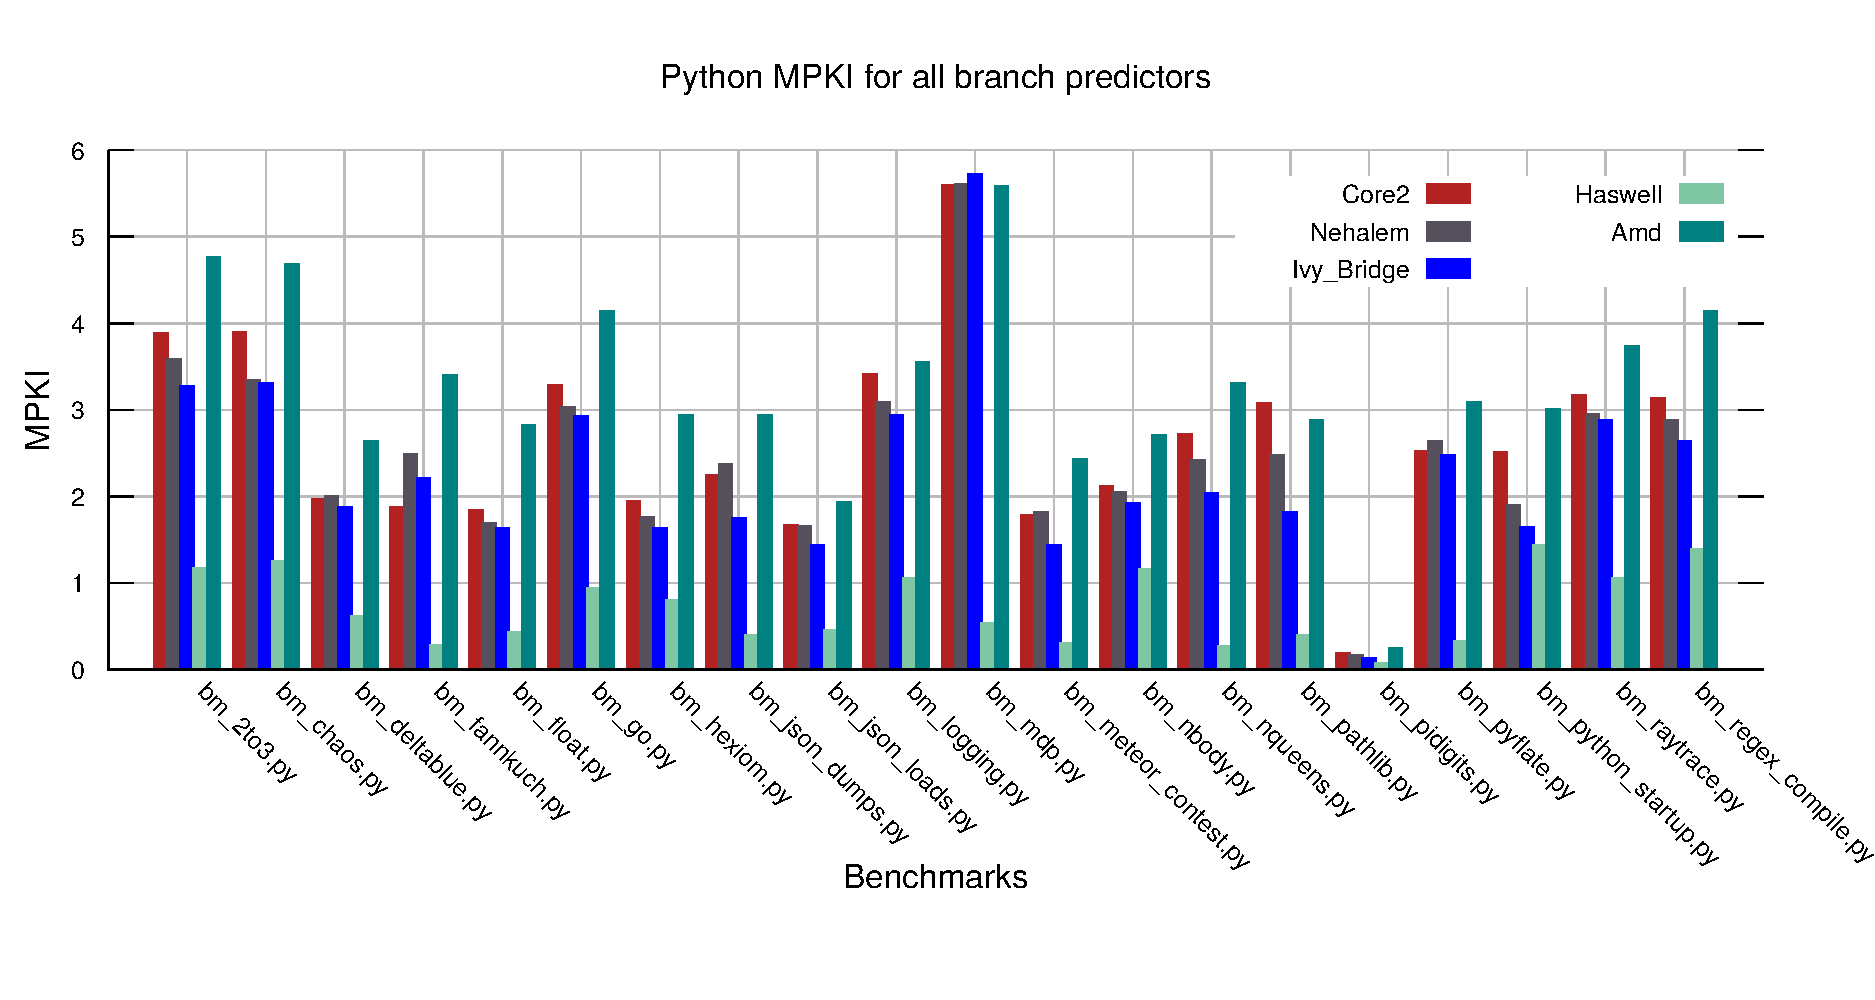
\includegraphics[width=11.5cm, height=6cm]{figures/python_MPKI.pdf}
    \end{figure}
\end{frame}

\begin{frame}{Javascript: Comparison of branch predictor's MPKI}
    \begin{figure}[t]
        \centering
        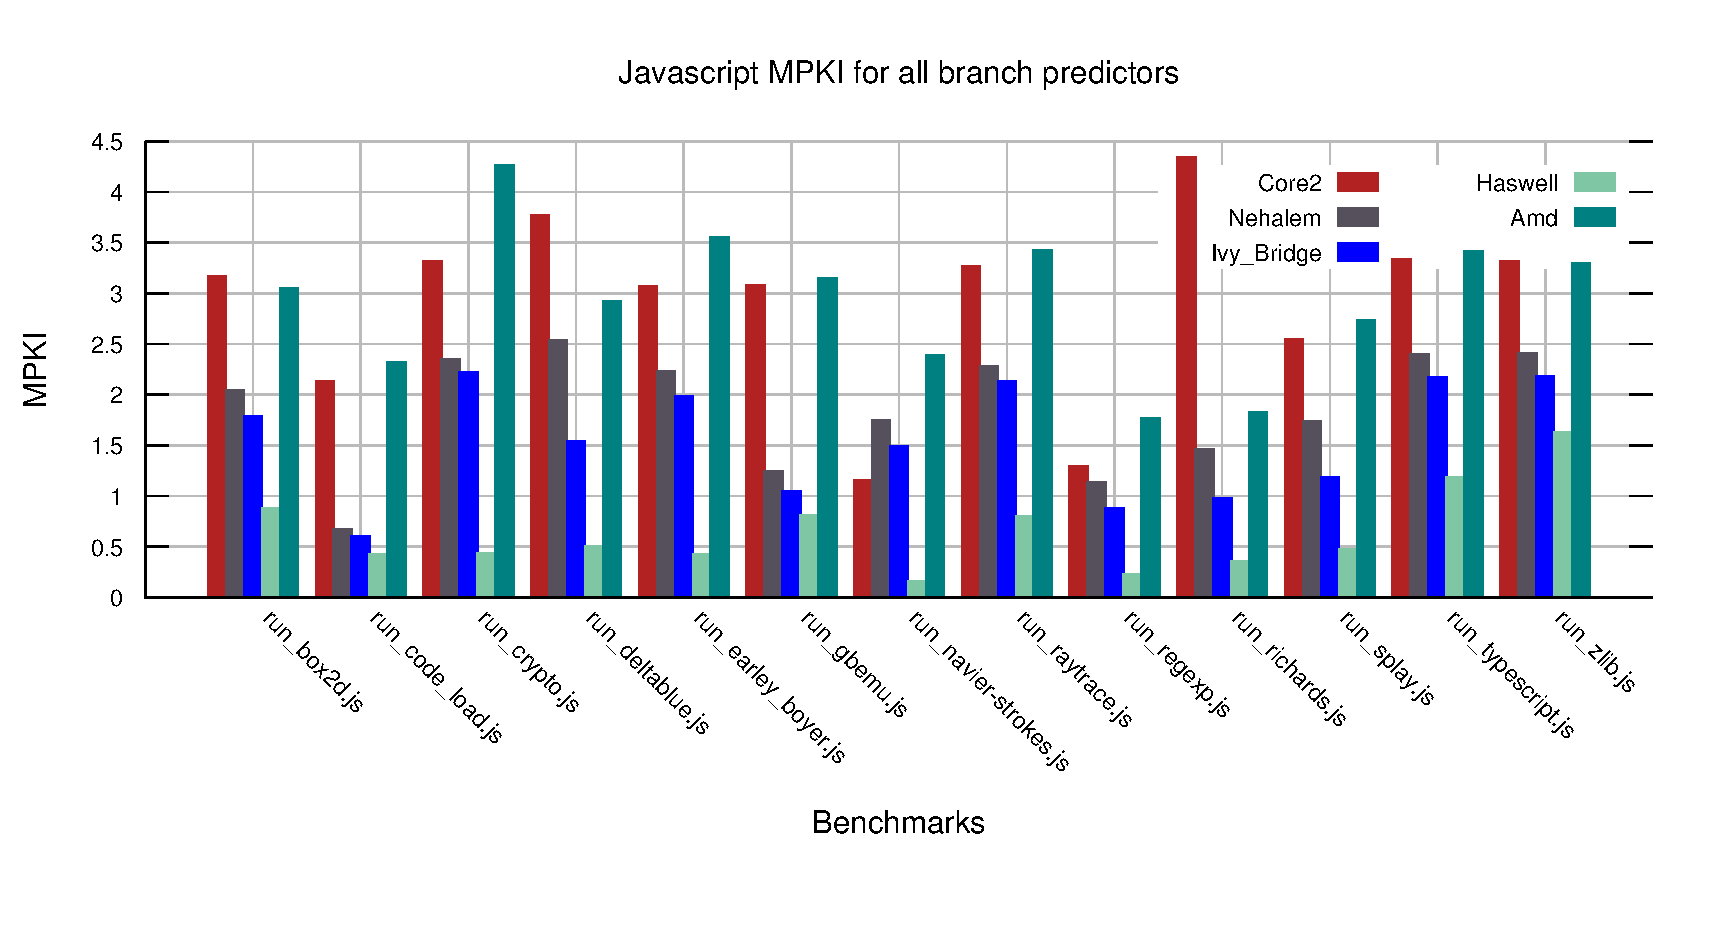
\includegraphics[width=11.5cm, height=6cm]{figures/javascript_MPKI.pdf}
    \end{figure}
\end{frame}

\begin{frame}{Java: Comparison of branch predictor's MPKI}
    \begin{figure}[t]
        \centering
        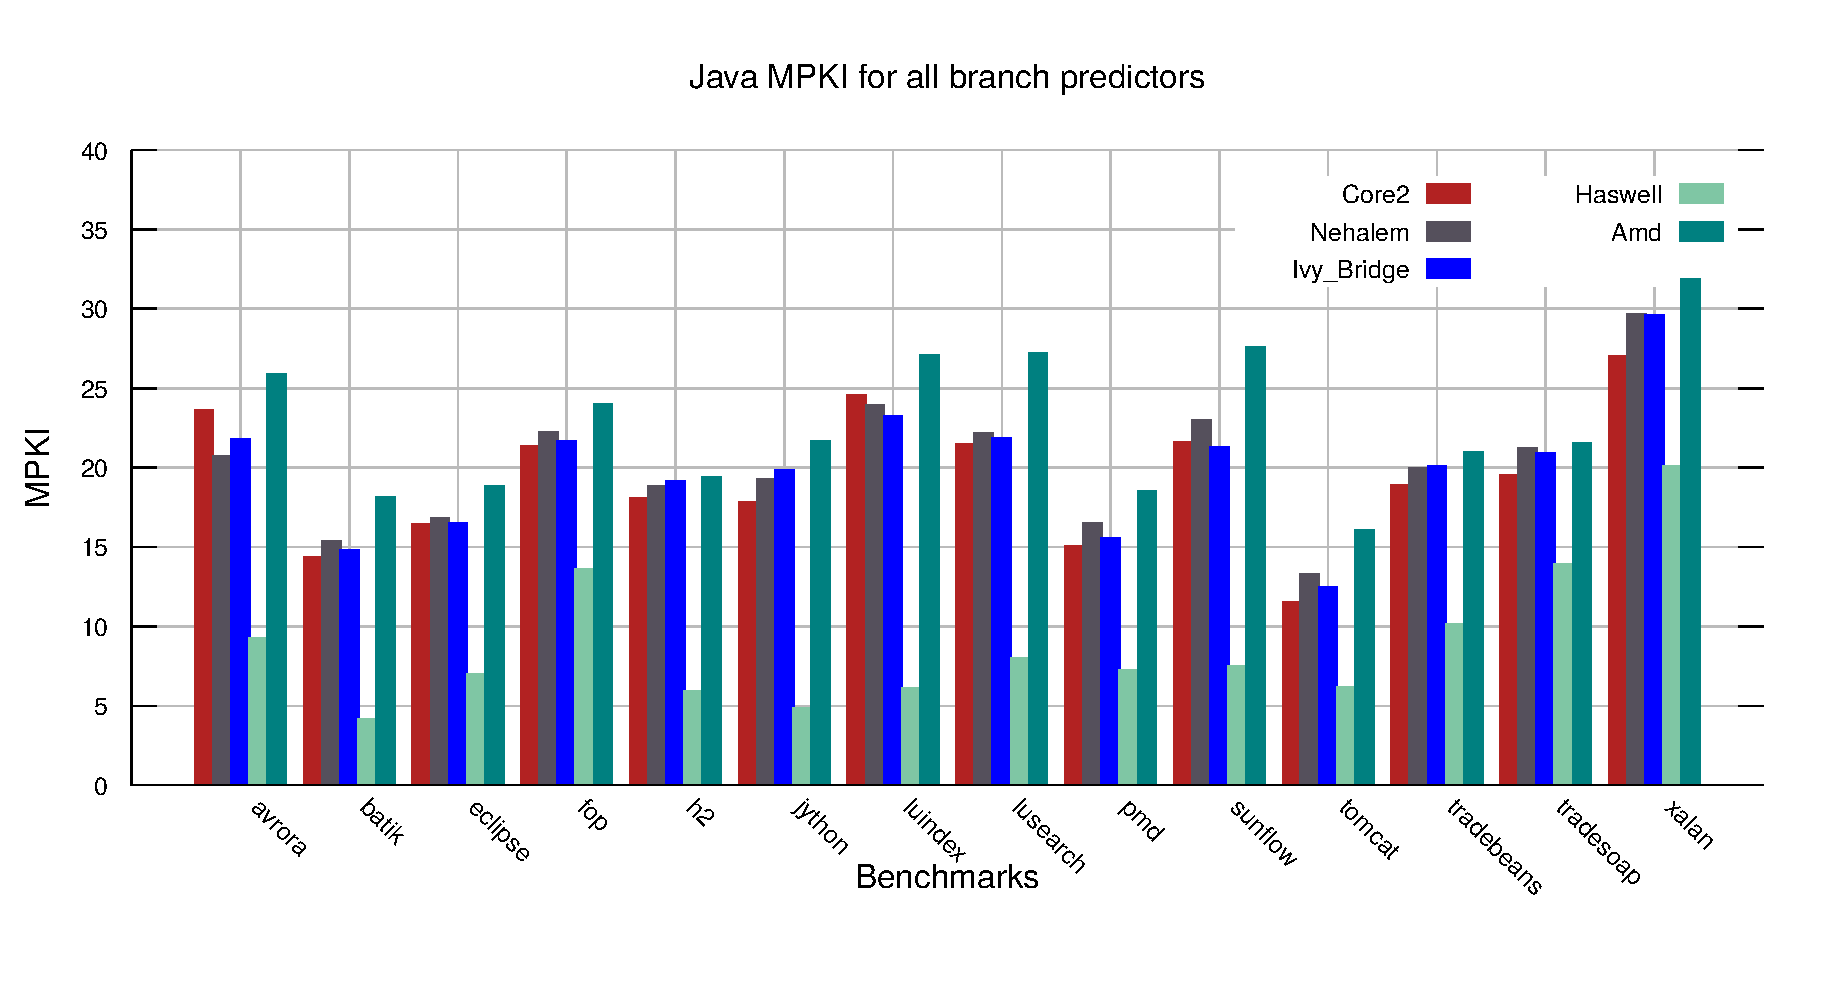
\includegraphics[width=11.5cm, height=6cm]{figures/java_MPKI.pdf}
    \end{figure}
\end{frame}

\begin{frame}{Python: Benchmarks Distributional characteristics}
	\begin{minipage}{\textwidth}
		\begin{figure}
        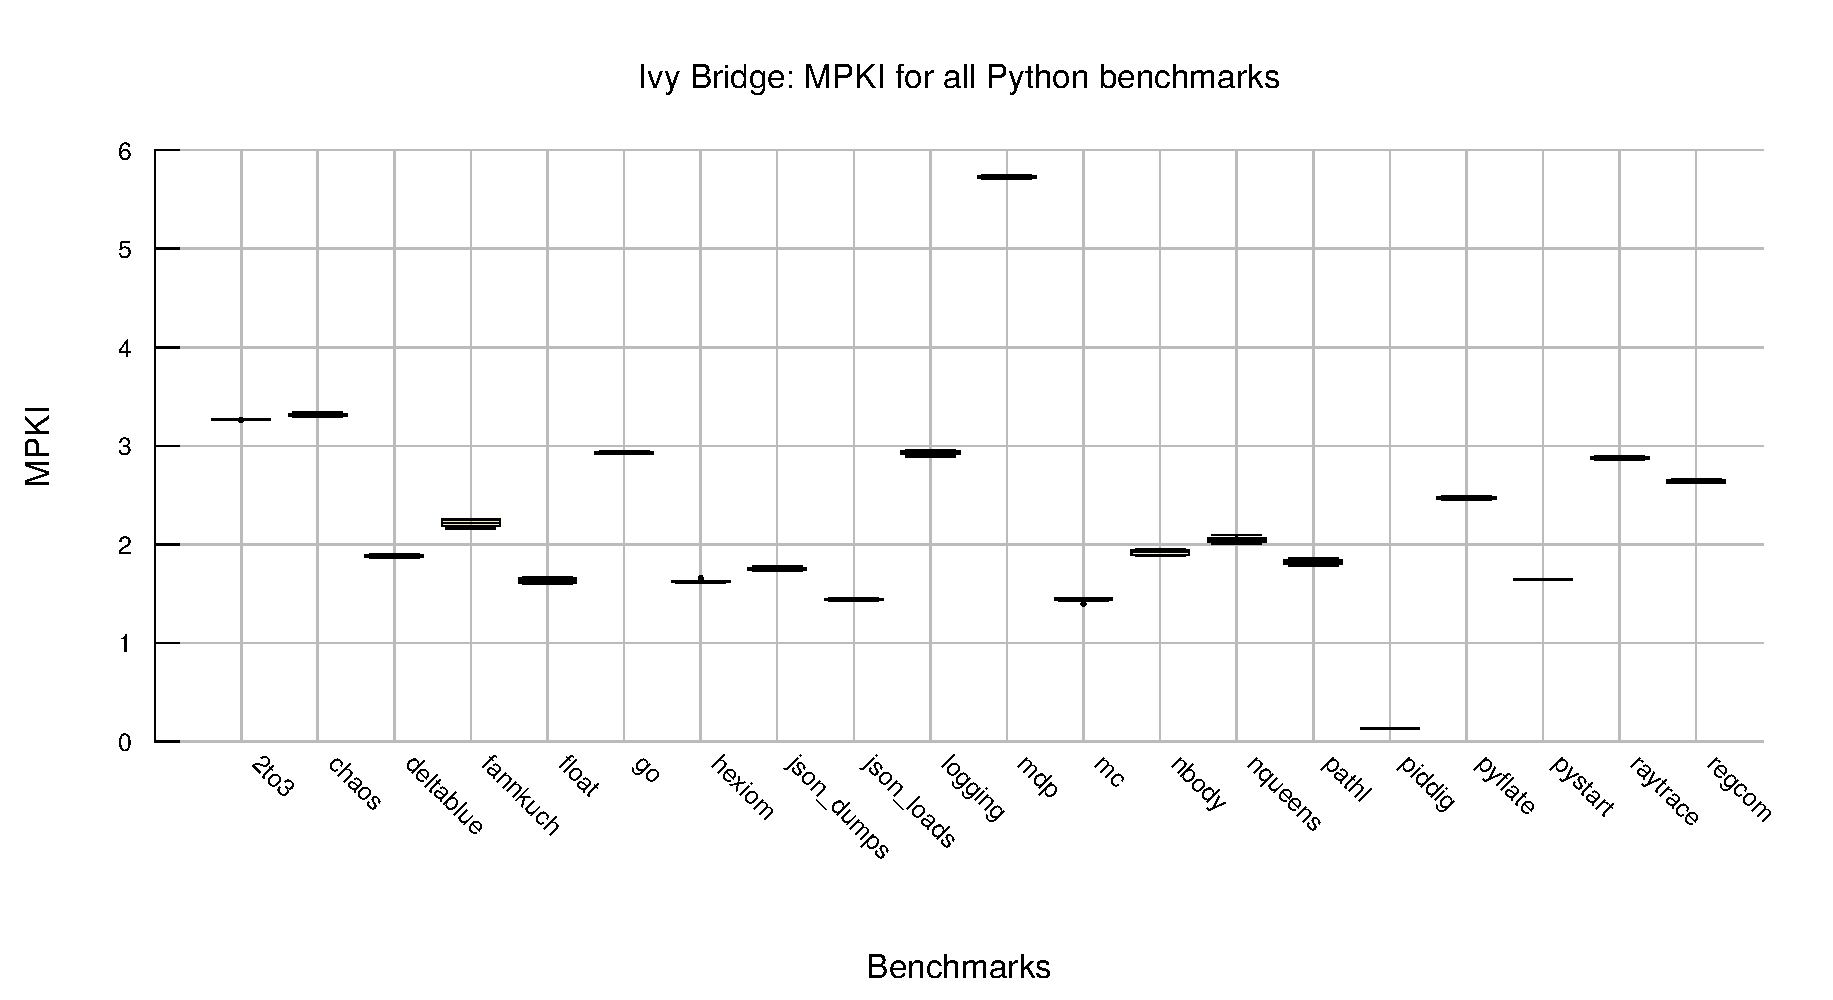
\includegraphics[width=8cm, height=4cm]{figures/python_box_ivy_bridge.pdf}
		\end{figure}
	\end{minipage}
		\begin{minipage}{\textwidth}
			\begin{figure}
				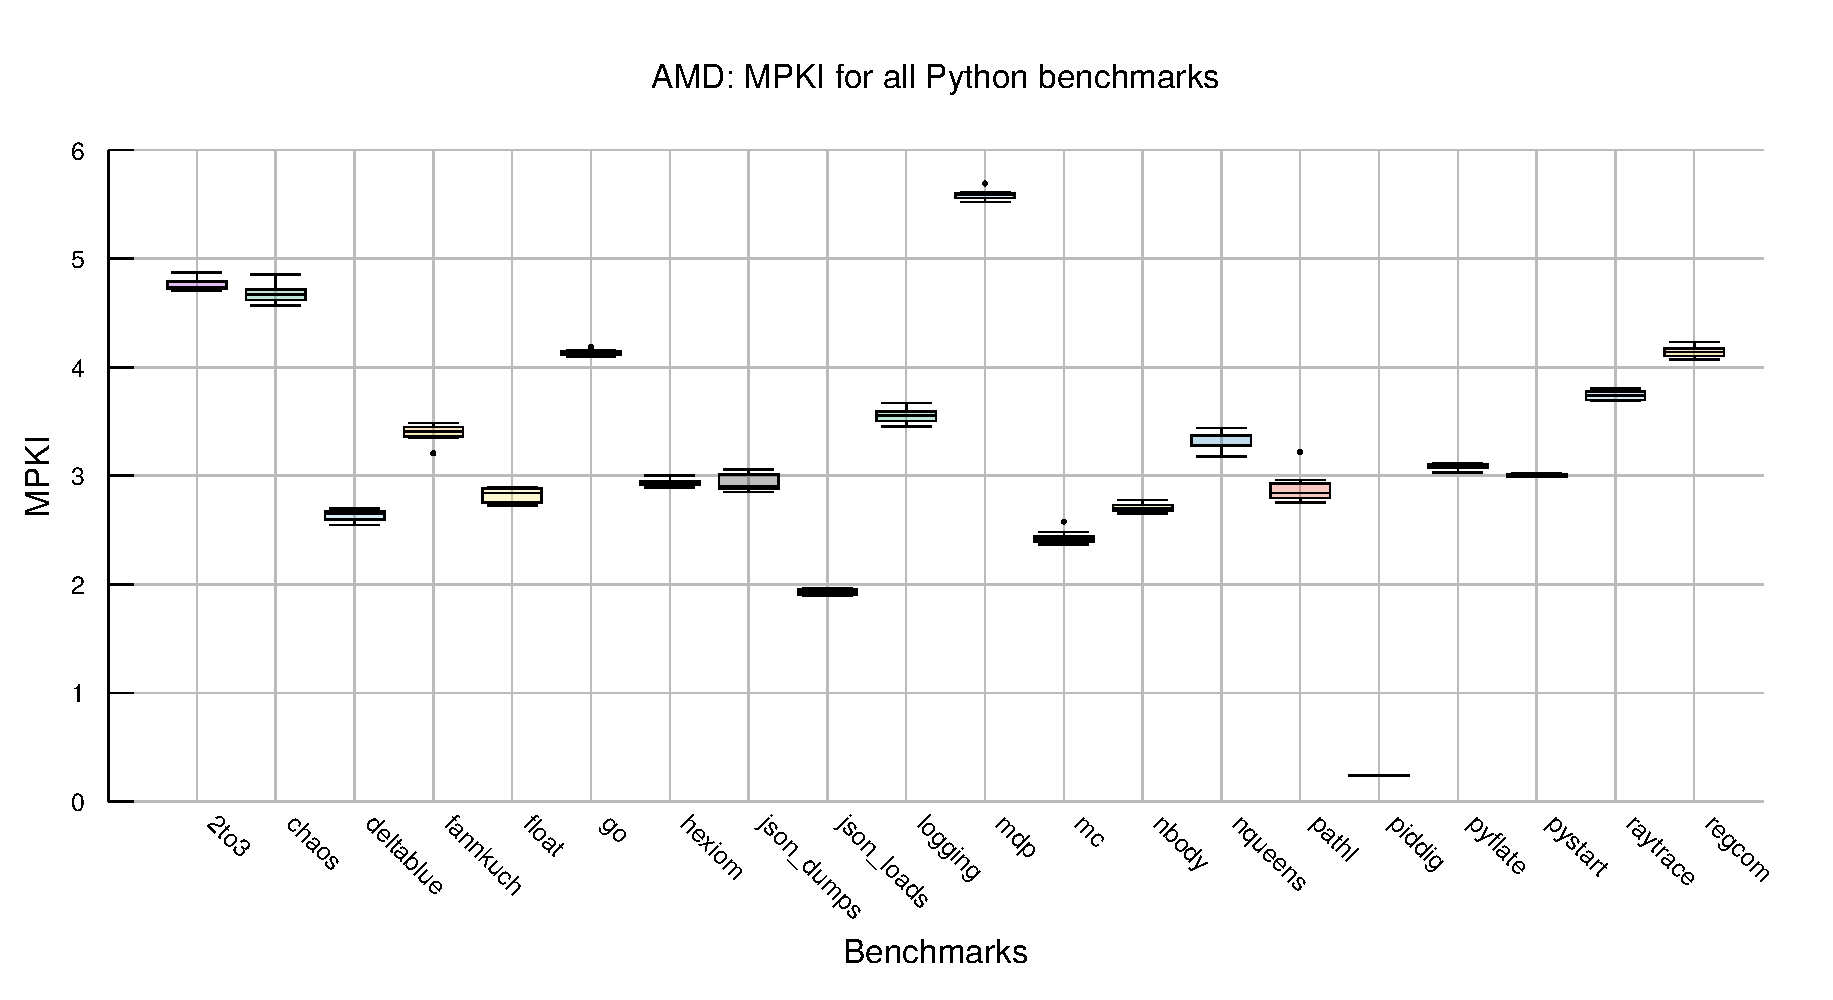
\includegraphics[width=8cm, height=4cm]{figures/python_box_amd.pdf}
			\end{figure}
		\end{minipage}
\end{frame}

\begin{frame}{Javascript: Benchmarks Distributional characteristics}
	\begin{minipage}{\textwidth}
		\begin{figure}
        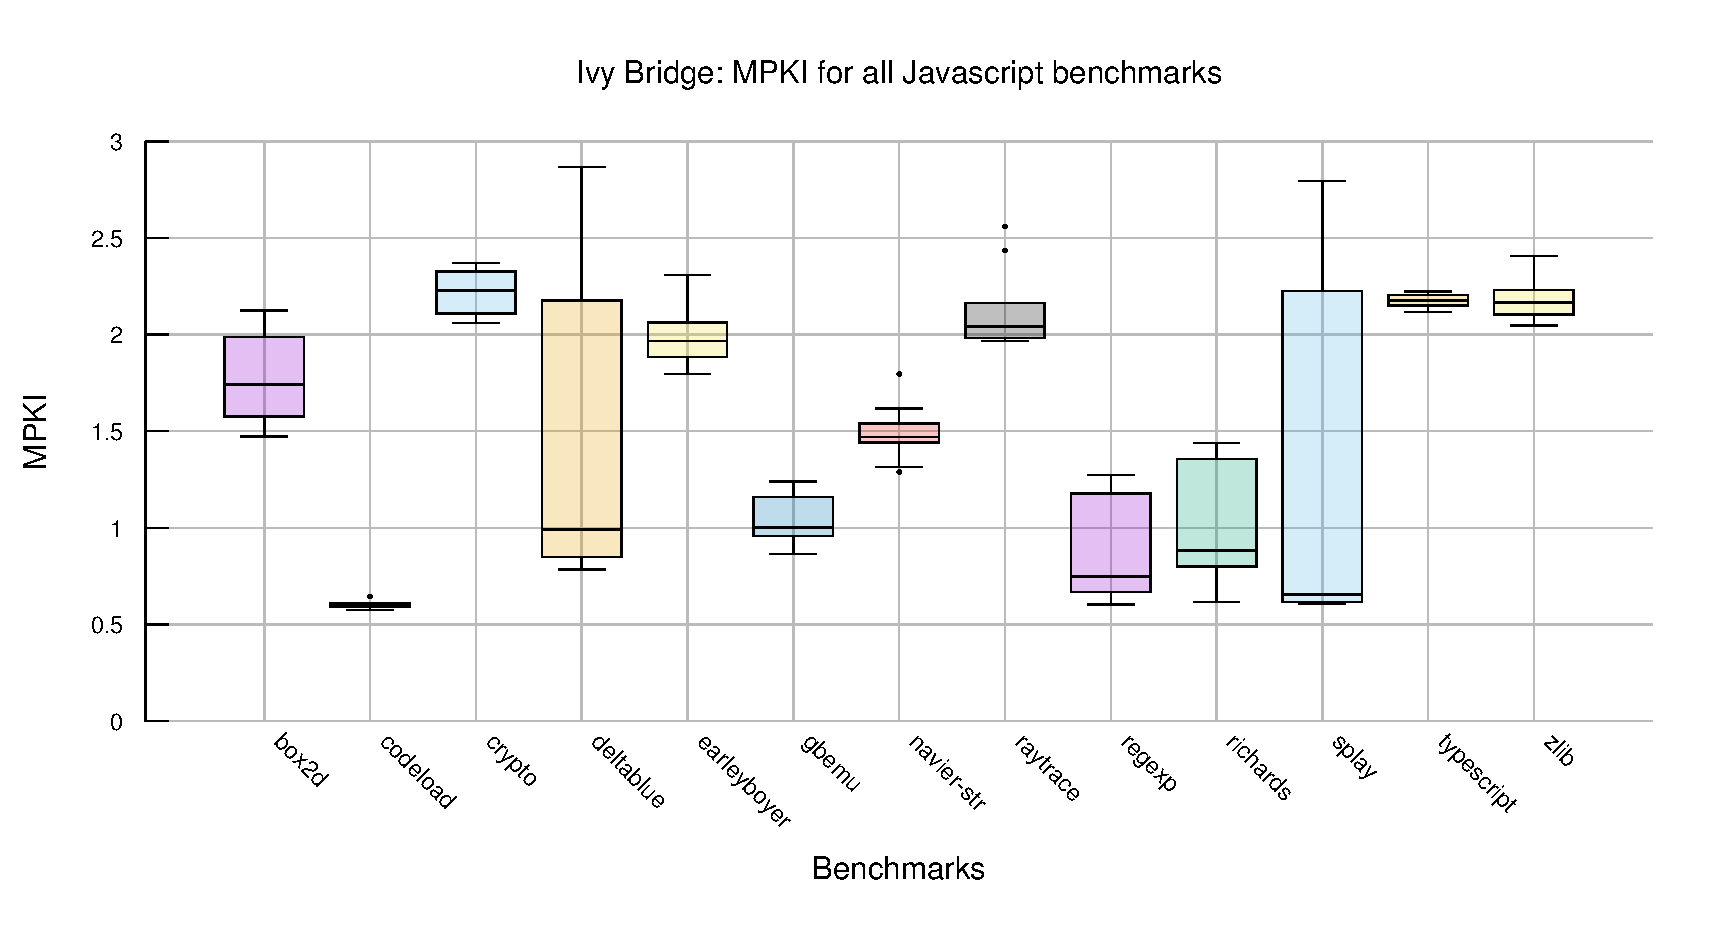
\includegraphics[width=8cm, height=4cm]{figures/javascript_box_ivy_bridge.pdf}
		\end{figure}
	\end{minipage}
		\begin{minipage}{\textwidth}
			\begin{figure}
				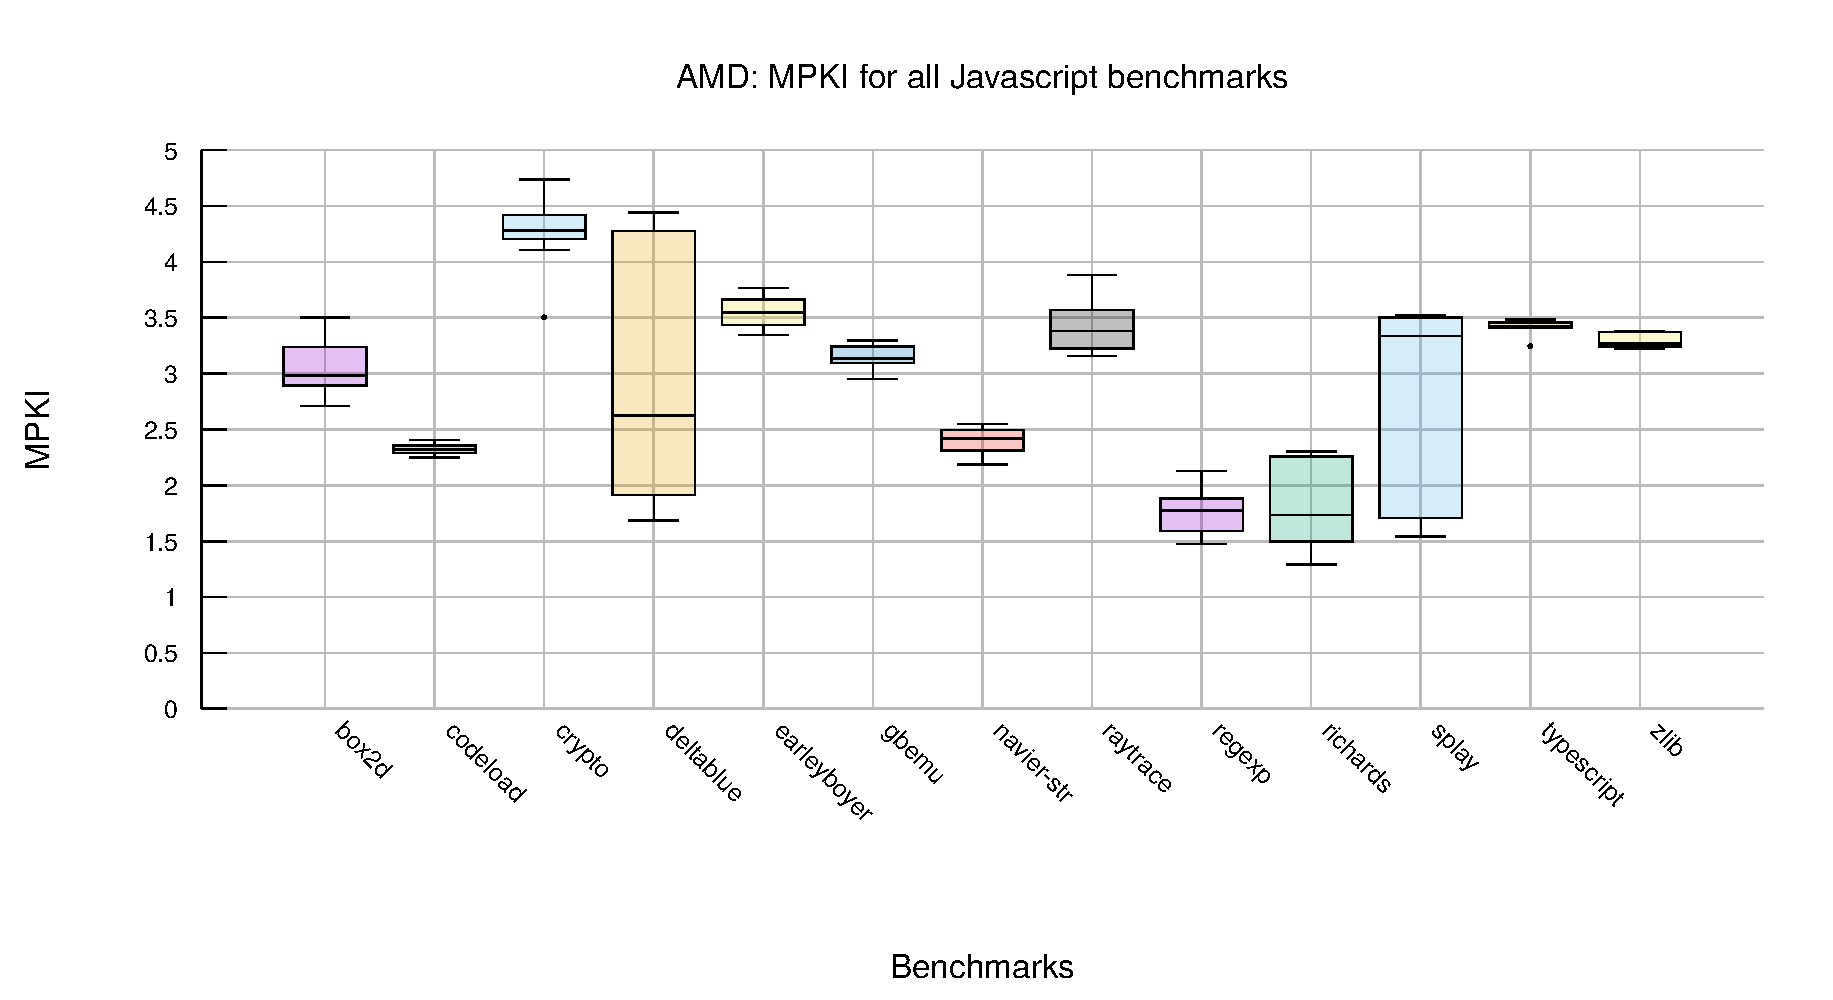
\includegraphics[width=8cm, height=4cm]{figures/javascript_box_amd.pdf}
			\end{figure}
		\end{minipage}
\end{frame}

\begin{frame}{Java: Benchmarks Distributional characteristics}
	\begin{minipage}{\textwidth}
		\begin{figure}
        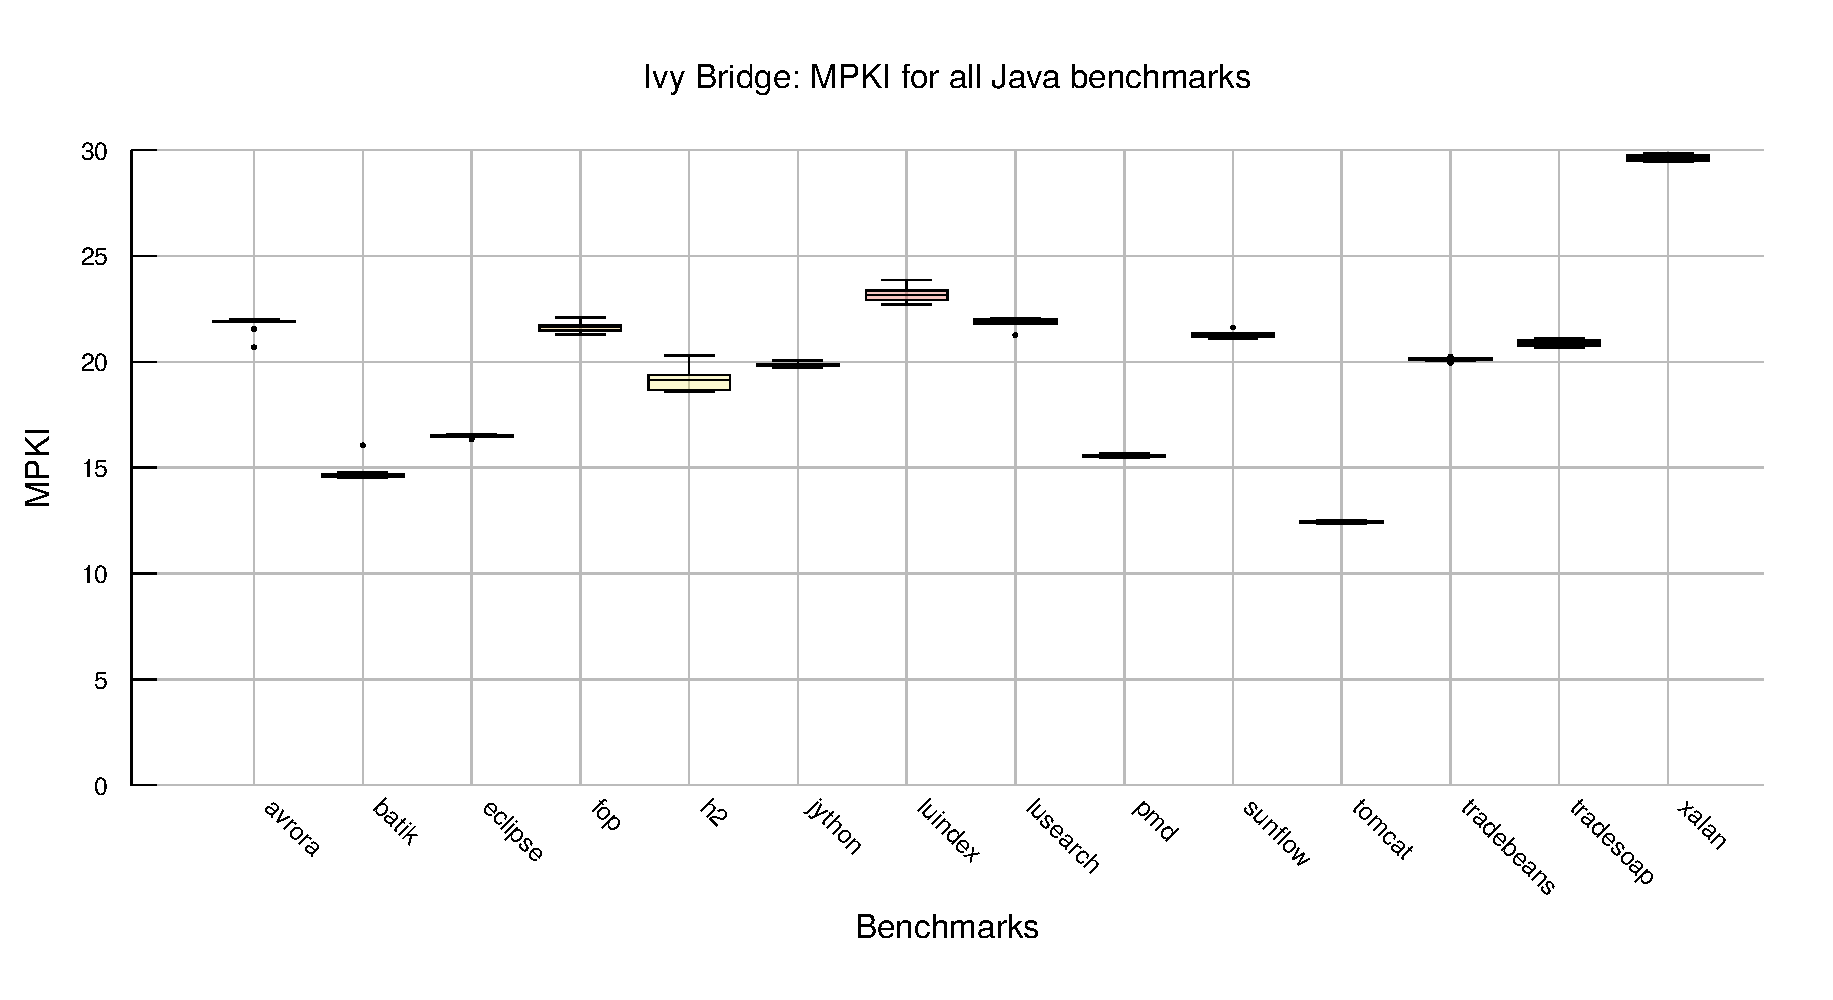
\includegraphics[width=8cm, height=4cm]{figures/java_box_ivy_bridge.pdf}
		\end{figure}
	\end{minipage}
		\begin{minipage}{\textwidth}
			\begin{figure}
				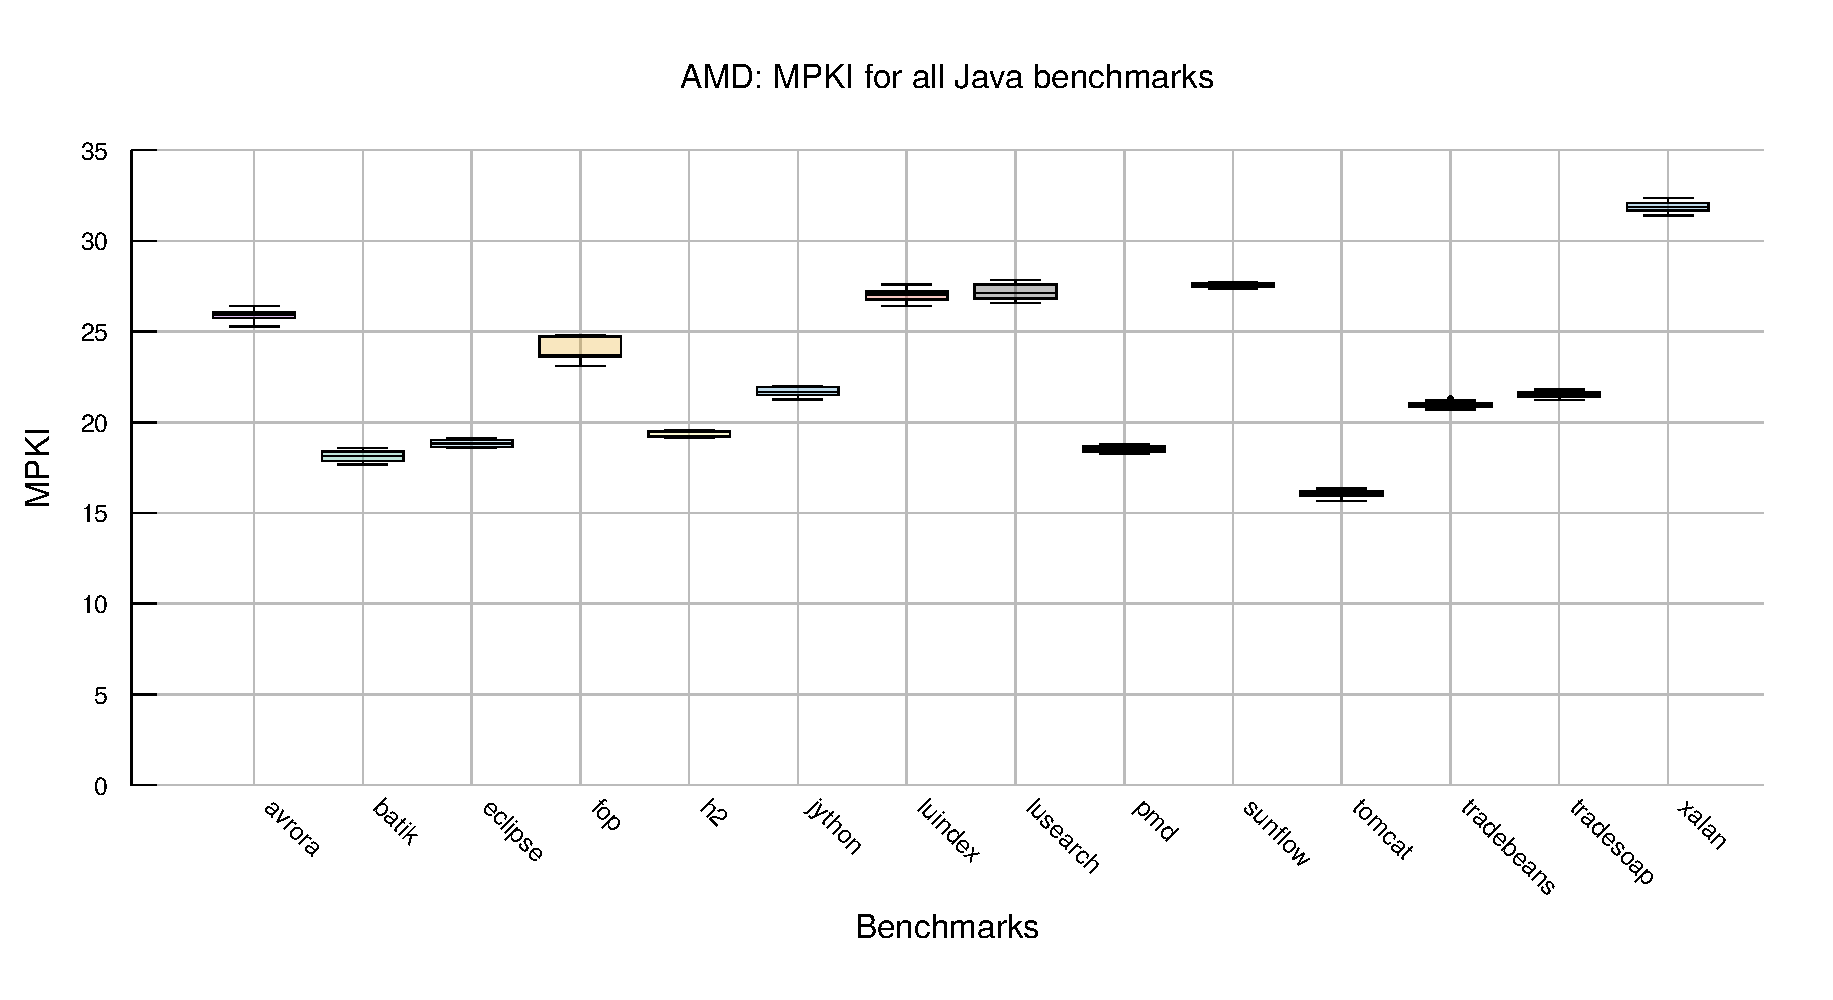
\includegraphics[width=8cm, height=4cm]{figures/java_box_amd.pdf}
			\end{figure}
		\end{minipage}
\end{frame}
%--------------------------------------------------------------------
% Conclusions
%--------------------------------------------------------------------
\section{Future work \& Summary}
\begin{frame}{What to do next!}
	\begin{itemize}
		\item {Isolate the mis-predictions created by VMs}
		\begin{itemize}
			\item{More accurate numbers of interpreter's mis-predictions}
			\item{Exclude the mis-predictions that produced by the VM}
		\end{itemize}
		\item {Run different versions/implementations of interpreters\\\small (i.e. python2.7 vs python3.6 or rhino vs spidermonkey)}
			\begin{itemize}
				\item{Determine the cause of mis-prediction accuracy improvement:}
				\begin{itemize}
						\item {Interpreters implementation}
						\item {Branch prediction accuracy}
				\end{itemize}
			\end{itemize}
	\end{itemize}
\end{frame}
\begin{frame}{Summary}
	\begin{itemize}
	\item{}
	\end{itemize}
\end{frame}
%--------------------------------------------------------------------
% Last Slide
%--------------------------------------------------------------------
\begin{frame}[standout] 
    \huge \textlatin{Thanks you! }\\
    \large \textlatin{Any questions? }
    \begin{figure}
    	
\includegraphics[width=1.5cm, height=1.5cm]{figures/questions.png}
    \end{figure}
\end{frame}
\end{document}
